\supplementarysection

\begin{figure}
    \centering
    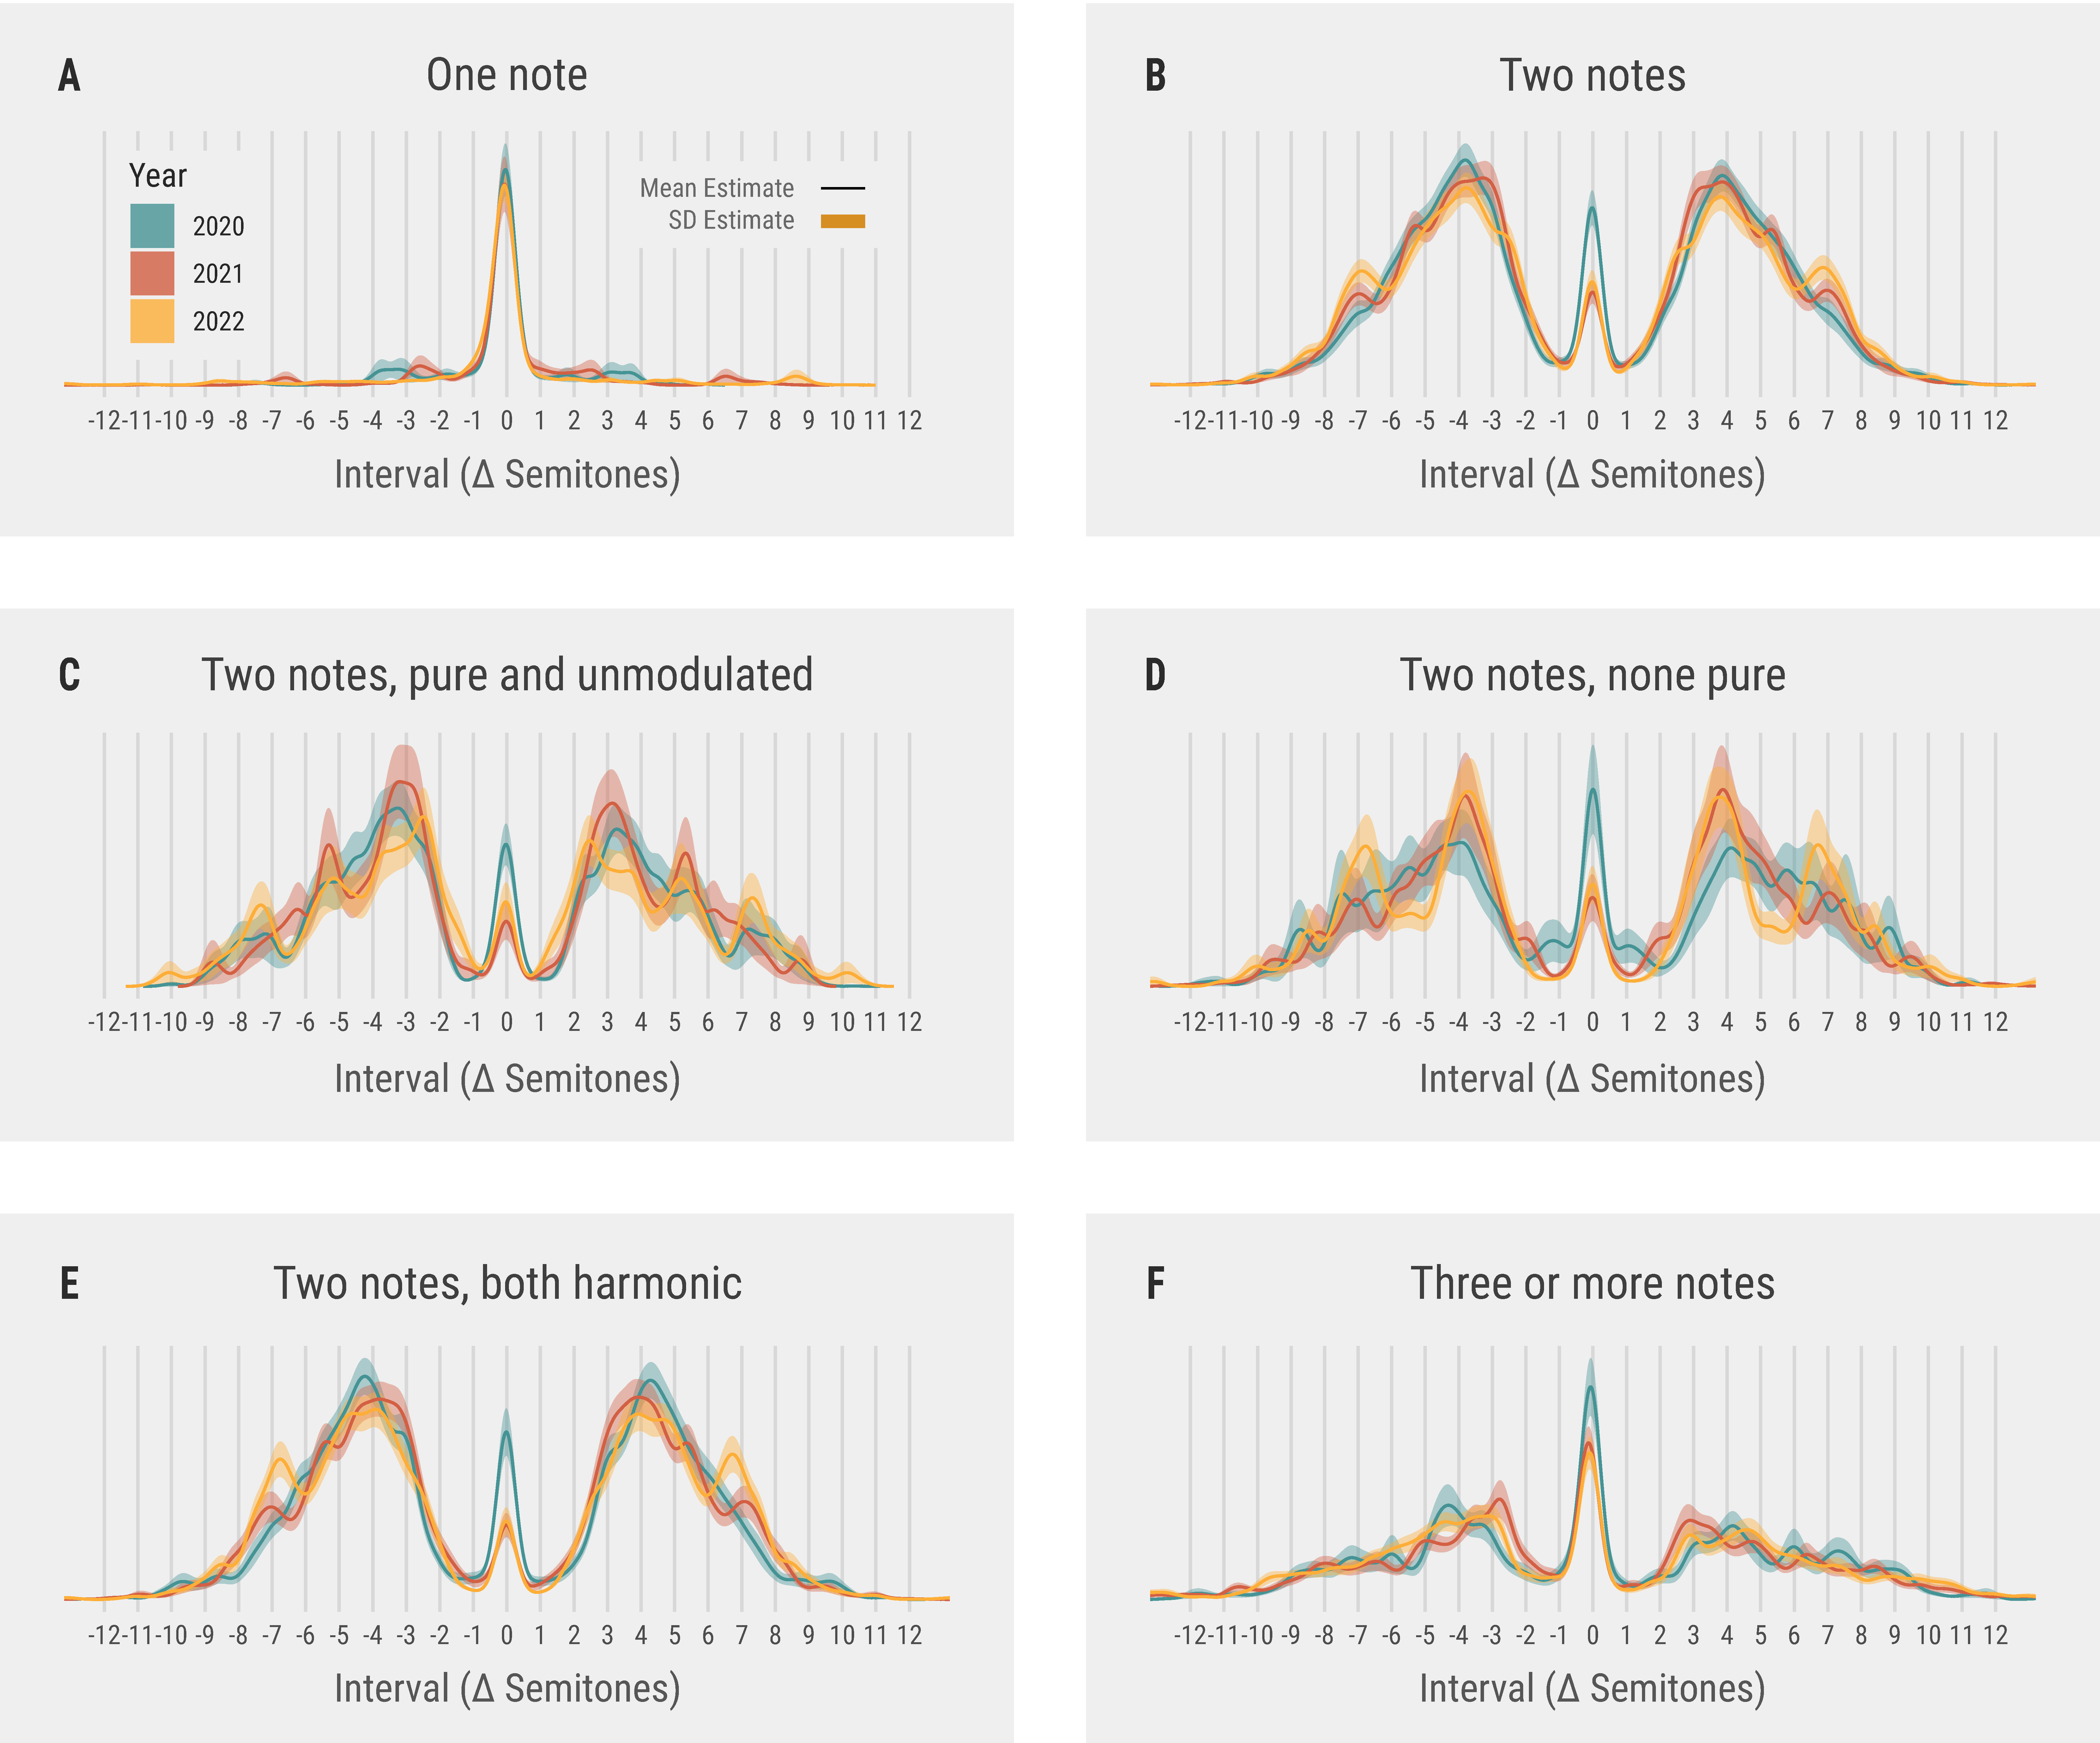
\includegraphics[width=\linewidth]{figures/chapter_5/melodic-songtypes-byyear.pdf}
    \mycaption{Kernel density estimates of the distribution of melodic intervals across a typology of songs in different years}{
    In this figure, we categorize songs into distinct types based on the number of notes they contain and their spectral properties and plot the estimated density distribution of melodic intervals, measured in semitones and spanning the octave (ascending and descending). Colours represent separate years in our study. 
    
    (A) One note: Songs consisting of a single note repeated rhythmically.
    (B) Two notes: All songs composed of two different, alternating notes.
    (C) Two notes, pure and unmodulated: Songs with two notes, each consisting of a single stable, pure, unmodulated tone.
    (D) Two notes, none pure: All two-note songs where neither note is pure and unmodulated.
    (E) Two notes, both harmonic: Songs featuring two notes, both of which have harmonic components.
    (F) Three or more notes: Songs comprising three or more notes. There are few three-note melodies, so we did not split these by spectral or modulation properties.
    }
    \label{c5_fig:melodic-byyear}
\end{figure}

